\documentclass{article}
\usepackage[utf8]{inputenc}
\usepackage[top=1in]{geometry}
\usepackage{tikz}
\usetikzlibrary{circuits.logic.US,positioning,calc} 
\usepackage{graphicx}
\usepackage{booktabs}
\usepackage{amsmath}
\usepackage[colorlinks]{hyperref}
% Calligraphic fonts
\newcommand{\calA}{{\cal A}}
\newcommand{\calB}{{\cal B}}
\newcommand{\calC}{{\cal C}}
\newcommand{\calD}{{\cal D}}
\newcommand{\calE}{{\cal E}}
\newcommand{\calF}{{\cal F}}
\newcommand{\calG}{{\cal G}}
\newcommand{\calH}{{\cal H}}
\newcommand{\calI}{{\cal I}}
\newcommand{\calJ}{{\cal J}}
\newcommand{\calK}{{\cal K}}
\newcommand{\calL}{{\cal L}}
\newcommand{\calM}{{\cal M}}
\newcommand{\calN}{{\cal N}}
\newcommand{\calO}{{\cal O}}
\newcommand{\calP}{{\cal P}}
\newcommand{\calQ}{{\cal Q}}
\newcommand{\calR}{{\cal R}}
\newcommand{\calS}{{\cal S}}
\newcommand{\calT}{{\cal T}}
\newcommand{\calU}{{\cal U}}
\newcommand{\calV}{{\cal V}}
\newcommand{\calW}{{\cal W}}
\newcommand{\calX}{{\cal X}}
\newcommand{\calY}{{\cal Y}}
\newcommand{\calZ}{{\cal Z}}

% Sets:
\newcommand{\setA}{\textsf{A}}
\newcommand{\setB}{\textsf{B}}
\newcommand{\setC}{\textsf{C}}
\newcommand{\setD}{\textsf{D}}
\newcommand{\setE}{\textsf{E}}
\newcommand{\setF}{\textsf{F}}
\newcommand{\setG}{\textsf{G}}
\newcommand{\setH}{\textsf{H}}
\newcommand{\setI}{\textsf{I}}
\newcommand{\setJ}{\textsf{J}}
\newcommand{\setK}{\textsf{K}}
\newcommand{\setL}{\textsf{L}}
\newcommand{\setM}{\textsf{M}}
\newcommand{\setN}{\textsf{N}}
\newcommand{\setO}{\textsf{O}}
\newcommand{\setP}{\textsf{P}}
\newcommand{\setQ}{\textsf{Q}}
\newcommand{\setR}{\textsf{R}}
\newcommand{\setS}{\textsf{S}}
\newcommand{\setT}{\textsf{T}}
\newcommand{\setU}{\textsf{U}}
\newcommand{\setV}{\textsf{V}}
\newcommand{\setW}{\textsf{W}}
\newcommand{\setX}{\textsf{X}}
\newcommand{\setY}{\textsf{Y}}
\newcommand{\setZ}{\textsf{Z}}

% Vectors
\newcommand{\bfa}{\mathbf{a}}
\newcommand{\bfb}{\mathbf{b}}
\newcommand{\bfc}{\mathbf{c}}
\newcommand{\bfd}{\mathbf{d}}
\newcommand{\bfe}{\mathbf{e}}
\newcommand{\bff}{\mathbf{f}}
\newcommand{\bfg}{\mathbf{g}}
\newcommand{\bfh}{\mathbf{h}}
\newcommand{\bfi}{\mathbf{i}}
\newcommand{\bfj}{\mathbf{j}}
\newcommand{\bfk}{\mathbf{k}}
\newcommand{\bfl}{\mathbf{l}}
\newcommand{\bfm}{\mathbf{m}}
\newcommand{\bfn}{\mathbf{n}}
\newcommand{\bfo}{\mathbf{o}}
\newcommand{\bfp}{\mathbf{p}}
\newcommand{\bfq}{\mathbf{q}}
\newcommand{\bfr}{\mathbf{r}}
\newcommand{\bfs}{\mathbf{s}}
\newcommand{\bft}{\mathbf{t}}
\newcommand{\bfu}{\mathbf{u}}
\newcommand{\bfv}{\mathbf{v}}
\newcommand{\bfw}{\mathbf{w}}
\newcommand{\bfx}{\mathbf{x}}
\newcommand{\bfy}{\mathbf{y}}
\newcommand{\bfz}{\mathbf{z}}


\newcommand{\bfalpha}{\boldsymbol{\alpha}}
\newcommand{\bfbeta}{\boldsymbol{\beta}}
\newcommand{\bfgamma}{\boldsymbol{\gamma}}
\newcommand{\bfdelta}{\boldsymbol{\delta}}
\newcommand{\bfepsilon}{\boldsymbol{\epsilon}}
\newcommand{\bfzeta}{\boldsymbol{\zeta}}
\newcommand{\bfeta}{\boldsymbol{\eta}}
\newcommand{\bftheta}{\boldsymbol{\theta}}
\newcommand{\bfiota}{\boldsymbol{\iota}}
\newcommand{\bfkappa}{\boldsymbol{\kappa}}
\newcommand{\bflambda}{\boldsymbol{\lambda}}
\newcommand{\bfmu}{\boldsymbol{\mu}}
\newcommand{\bfnu}{\boldsymbol{\nu}}
\newcommand{\bfomicron}{\boldsymbol{\omicron}}
\newcommand{\bfpi}{\boldsymbol{\pi}}
\newcommand{\bfrho}{\boldsymbol{\rho}}
\newcommand{\bfsigma}{\boldsymbol{\sigma}}
\newcommand{\bftau}{\boldsymbol{\tau}}
\newcommand{\bfupsilon}{\boldsymbol{\upsilon}}
\newcommand{\bfphi}{\boldsymbol{\phi}}
\newcommand{\bfchi}{\boldsymbol{\chi}}
\newcommand{\bfpsi}{\boldsymbol{\psi}}
\newcommand{\bfomega}{\boldsymbol{\omega}}
\newcommand{\bfxi}{\boldsymbol{\xi}}
\newcommand{\bfell}{\boldsymbol{\ell}}

% Matrices
\newcommand{\bfA}{\mathbf{A}}
\newcommand{\bfB}{\mathbf{B}}
\newcommand{\bfC}{\mathbf{C}}
\newcommand{\bfD}{\mathbf{D}}
\newcommand{\bfE}{\mathbf{E}}
\newcommand{\bfF}{\mathbf{F}}
\newcommand{\bfG}{\mathbf{G}}
\newcommand{\bfH}{\mathbf{H}}
\newcommand{\bfI}{\mathbf{I}}
\newcommand{\bfJ}{\mathbf{J}}
\newcommand{\bfK}{\mathbf{K}}
\newcommand{\bfL}{\mathbf{L}}
\newcommand{\bfM}{\mathbf{M}}
\newcommand{\bfN}{\mathbf{N}}
\newcommand{\bfO}{\mathbf{O}}
\newcommand{\bfP}{\mathbf{P}}
\newcommand{\bfQ}{\mathbf{Q}}
\newcommand{\bfR}{\mathbf{R}}
\newcommand{\bfS}{\mathbf{S}}
\newcommand{\bfT}{\mathbf{T}}
\newcommand{\bfU}{\mathbf{U}}
\newcommand{\bfV}{\mathbf{V}}
\newcommand{\bfW}{\mathbf{W}}
\newcommand{\bfX}{\mathbf{X}}
\newcommand{\bfY}{\mathbf{Y}}
\newcommand{\bfZ}{\mathbf{Z}}


\newcommand{\bfGamma}{\boldsymbol{\Gamma}}
\newcommand{\bfDelta}{\boldsymbol{\Delta}}
\newcommand{\bfTheta}{\boldsymbol{\Theta}}
\newcommand{\bfLambda}{\boldsymbol{\Lambda}}
\newcommand{\bfPi}{\boldsymbol{\Pi}}
\newcommand{\bfSigma}{\boldsymbol{\Sigma}}
\newcommand{\bfUpsilon}{\boldsymbol{\Upsilon}}
\newcommand{\bfPhi}{\boldsymbol{\Phi}}
\newcommand{\bfPsi}{\boldsymbol{\Psi}}
\newcommand{\bfOmega}{\boldsymbol{\Omega}}


% Blackboard Bold:
\newcommand{\bbA}{\mathbb{A}}
\newcommand{\bbB}{\mathbb{B}}
\newcommand{\bbC}{\mathbb{C}}
\newcommand{\bbD}{\mathbb{D}}
\newcommand{\bbE}{\mathbb{E}}
\newcommand{\bbF}{\mathbb{F}}
\newcommand{\bbG}{\mathbb{G}}
\newcommand{\bbH}{\mathbb{H}}
\newcommand{\bbI}{\mathbb{I}}
\newcommand{\bbJ}{\mathbb{J}}
\newcommand{\bbK}{\mathbb{K}}
\newcommand{\bbL}{\mathbb{L}}
\newcommand{\bbM}{\mathbb{M}}
\newcommand{\bbN}{\mathbb{N}}
\newcommand{\bbO}{\mathbb{O}}
\newcommand{\bbP}{\mathbb{P}}
\newcommand{\bbQ}{\mathbb{Q}}
\newcommand{\bbR}{\mathbb{R}}
\newcommand{\bbS}{\mathbb{S}}
\newcommand{\bbT}{\mathbb{T}}
\newcommand{\bbU}{\mathbb{U}}
\newcommand{\bbV}{\mathbb{V}}
\newcommand{\bbW}{\mathbb{W}}
\newcommand{\bbX}{\mathbb{X}}
\newcommand{\bbY}{\mathbb{Y}}
\newcommand{\bbZ}{\mathbb{Z}}




\title{Homework 4}
\author{Max marks: 100}
\date{Due on October 21, 2022, 12:00 noon, before class. Please submit in paper,
because it is easier to grade. Also submit a backup copy to brightspace. If you
are submitting code: submit the code on brightspace; submit compilation and
running instructions, test environment, and IO output in paper.}
\newtheorem{prob}{Problem}

\newcommand{\bx}{\bar{x}}
\newcommand{\by}{\bar{y}}
\newcommand{\bz}{\bar{z}}
\newcommand{\bA}{\bar{A}}
\newcommand{\bB}{\bar{B}}
\newcommand{\bC}{\bar{C}}
\begin{document}

\maketitle
You can choose to implement Quine-McCluskey in your favorite programming language
(C, C++, python, javascript etc). Or you can do the following problems by hand.
If you use any third-party code, please attribute the third-party code and
delineate your code clearly.
More than 50\% of the code should be your own.

\begin{prob}
  Use Quine-McCluskey method to find the minimal SOP for $f(x, y, z) = \sum m(2,
  3, 4, 5)$ (20 marks)
\end{prob}

\begin{prob}
  Use Quine-McCluskey method to find the minimal SOP for $f(x, y, z, w) = \sum
  m(0, 1, 4, 5, 12, 13)$ (20 marks)
\end{prob}

\begin{prob}
  Use Quine-McCluskey method to find the minimal SOP for $f(x, y, z, w) = \sum
  m(1, 5, 7, 8, 9, 13, 15) + d(4, 14)$ (20 marks).
\end{prob}

%\begin{prob}
%  A circuit with two outputs has to implement the following functions
%  \begin{align}
%    f(x_1, \dots, x_4) &= \sum m(0, 2, 4, 6, 7, 9) + d(10, 11)
%    \\
%    g(x_1, \dots, x_4) &= \sum m(2, 4, 9, 10, 15) + d(0, 13, 14)
%  \end{align}
%  Design a minimum-cost SOP circuit and compare its cost with combined cost of
%  two SOP circuits that implement $f$ and $g$ separately. Assume the input
%  variables in both complemented and uncomplemented forms. 
%\end{prob}

\begin{prob}
  Refer to the datasheet of Texas Instrument IC (Integrated circuit) \href{https://www.ti.com/lit/ds/symlink/sn74ls00.pdf}{SN74LS00} and
  \href{https://www.ti.com/lit/ds/symlink/sn74ls04.pdf}{SN74LS04}. SN74LS00 chip contains four two-input NAND gates. SN74LS04 contains
  six NOT gates. 
  Find the $V_{IH}$ and $V_{IL}$ in the ``recommended operating conditions''
  section and $V_{OH}$ and $V_{OL}$ in the ``electrical characteristic''
  section for both SN74LS00 and SN74LS04. In multiple values are given chose the ``TYP'' value, because we
  assume to operate the IC under ``NOM'' conditions.
  This is not to test you, but to relate this your knowledge to real
  world. If you are having trouble finding this information, please email me and
  I will send you the correct values. The next part is to test your understanding.
  Find noise margin high and
  noise margin low for the wire labeled $g$ following circuits (20 marks).
\end{prob}

Circuit A:

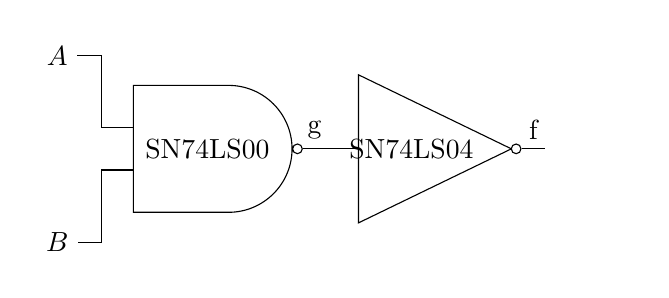
\begin{tikzpicture}[circuit logic US]
  \matrix[column sep=7mm]{
    \node (A) {$A$}; &  & & & \\
    & \node [nand gate] (AnandB) {SN74LS00}; &  \node [not gate] (f) {SN74LS04}; \\
    \node (B) {$B$}; & & & & \\
  };
  \draw (A.east) -- ++(right:3mm) |- (AnandB.input 1);
  \draw (B.east) -- ++(right:3mm) |- (AnandB.input 2);
  \draw (AnandB.output) to [edge label=g] ++(right:3mm) |- (f.input);

  \draw (f.output) to [edge label=f] ++(right:3mm);
\end{tikzpicture}

Circuit B:

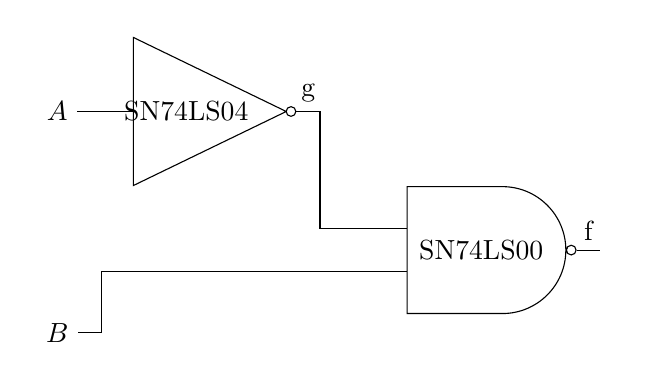
\begin{tikzpicture}[circuit logic US]
  \matrix[column sep=7mm]{
    \node (A) {$A$}; & \node [not gate] (notA) {SN74LS04}; & &\\
    & & & \node [nand gate] (notAnandB) {SN74LS00}; \\
    \node (B) {$B$}; & & & & \\
  };
  \draw (A.east)  -- ++(right:3mm) |- (notA.input);
  \draw (notA.output) to [edge label=g] ++(right:3mm) |- (notAnandB.input 1);
  \draw (B.east) -- ++(right:3mm) |- (notAnandB.input 2);

  \draw (notAnandB.output) to [edge label=f] ++(right:3mm);
\end{tikzpicture}

\begin{prob}
  Design a 2-input OR gate using 
  \begin{enumerate}
    \item nMOS transistors (5 marks).
    \item CMOS technology (5 marks).
    \item negative logic and CMOS technology (10 marks).
  \end{enumerate}
\end{prob}
%\bibliography{main}
%\bibliographystyle{plain}
\end{document}
